\documentclass[11pt]{amsart}
\usepackage[T1]{fontenc}
\usepackage{lmodern}
\usepackage{mathtools,amssymb,graphicx,booktabs,enumitem}
\usepackage[hidelinks]{hyperref}
\hypersetup{
  pdftitle={Shape-Controlled Gravitational Propulsion: Iso-Inertial Hopf Holonomy, Three-Dimensional J2 Symmetry Breaking, and Mechanical-Hub Hardware Sizing},
  pdfauthor={Ergentics},
  pdfkeywords={shape-controlled gravitational propulsion, Hopf fibration, geometric phase, J2 oblateness, space tethers, mechanical hub}
}
\pdfinfo{/Producer () /Creator ()}
\usepackage{microtype}
\numberwithin{equation}{section}
\theoremstyle{plain}
\newtheorem{theorem}{Theorem}[section]
\newtheorem{proposition}[theorem]{Proposition}
\newtheorem{lemma}[theorem]{Lemma}
\newtheorem{corollary}[theorem]{Corollary}
\theoremstyle{definition}\newtheorem{definition}[theorem]{Definition}
\theoremstyle{remark}\newtheorem{remark}[theorem]{Remark}
\newcommand{\R}{\mathbb{R}}
\newcommand{\C}{\mathbb{C}}
\newcommand{\Z}{\mathbb{Z}}
\newcommand{\SO}{\mathrm{SO}}
\newcommand{\ctag}[1]{\textup{\textsf{\scriptsize[#1]}}}
\emergencystretch=3em
\raggedbottom

\title[Shape-Controlled Gravitational Propulsion]{Shape-Controlled Gravitational Propulsion: Iso-Inertial Hopf Holonomy, Three-Dimensional $J_2$ Symmetry Breaking, and Mechanical-Hub Hardware Sizing}
\author{Ergentics}
\date{November 2026}
\subjclass[2020]{Primary 70F15, 70E15; Secondary 70G45, 70K65, 70Q05}
\keywords{gravitational swinging, Hopf fibration, Guichardet--Shapere--Wilczek holonomy, oblate $J_2$ perturbation, space tethers, mechanical differential hub}

\begin{document}
\begin{abstract}
We present a reconciled, self-contained synthesis of planar and three-dimensional shape-controlled gravitational propulsion for an iso-inertial three-mass spacecraft triad, unifying and repairing the Horizon clean-room manuscripts \texttt{WP~030} and \texttt{WP~031} under a single set of physical constants and open, reproducible simulations. Five structural issues uncovered during cross-agent verification are resolved in place: (i)~the exact finite-size tidal acceleration is evaluated via a cancellation-free factored formulation eliminating catastrophic IEEE-754 double-precision loss below $\epsilon = L/R \lesssim 10^{-7}$; (ii)~the planar iso-inertial Hopf holonomy is formulated in the equilateral-pole Jacobi basis $w_\pm = (z_1 \pm i z_2)/\sqrt{2}$, yielding an exact physical rotation $\Delta\theta_{\mathrm{phys}} = -90^\circ$ while keeping all inter-mass separations strictly positive ($\min d_{ij} = \sqrt{2-\sqrt{3}}\,L \approx 0.5176\,L$); (iii)~the closed-form iso-inertial kinetic-energy wall $K_{\mathrm{int}}(q)/(\tfrac12 I_0 \Omega^2) = q^2/(1-q^2)$ (Theorem~G1) bounds high-amplitude pumping; (iv)~all safe-perigee mission metrics are standardized to WGS84 equatorial Earth radius $R_\oplus = 6{,}378.137\text{ km}$ ($r_p = 6{,}978.137\text{ km}$, optimal eccentricity $e^* = 0.281702$, headline $\Delta v/\mathrm{yr} = 199.89\text{ m/s/yr}$ at $L=20\text{ km}$), and 3D oblate $J_2$ symmetry breaking is isolated by subtracting an identical $L=0$ point-mass control while tracking coupled axial spin $J_z = L_z + S_z$ to $< 10^{-12}$; and (v)~consistent polar inertia $I_0 = \frac23 M L^2$ establishes an $I_0$-invariant $9.85\times$ minimum electrical regeneration-to-orbital heat floor ($15.16\times$ at $q=0.50$, Theorem~G4), driving the flight baseline to a spin-tensioned Hopf triad with a coupled mechanical spring-drum hub that reduces waste heat by $22.4\times$ (from $312.2\text{ W}$ to $13.9\text{ W}$) at a hardware mass of $45.4\text{ kg}$ versus $100.5\text{ kg}$ wet for a 5-year Hall thruster. All numerical claims are independently verified by an open, zero-dependency Python simulator (\texttt{piece1\_sim.py}, 7/7 deterministic, runtime, and keyed stochastic gates passing).
\end{abstract}
\maketitle

\section{Introduction and Synthesis Scope}
Propellantless orbital modification by cyclic redistribution of a spacecraft's mass distribution in a non-uniform gravitational field---often called \emph{gravitational swinging}---was pioneered for tethered dumbbells by Martinez-Sanchez and Gavit \cite{martinez1987} and Landis \cite{landis1990,landis1992}, formalized in general relativity by Wisdom \cite{wisdom2003} and Gu\'eron, Maia, and Matsas \cite{gueron2006}, and embedded in the gauge theory of deformable bodies by Guichardet \cite{guichardet1984}, Iwai \cite{iwai1987}, Shapere and Wilczek \cite{shapere1989a,shapere1989b}, and Montgomery \cite{montgomery1993}. Unlike a rigid dumbbell, whose principal moments of inertia change during deployment and therefore tumble under gravity-gradient torque, a three-mass spacecraft can execute closed loops on its iso-inertial shape sphere $S^2$, combining zero-angular-momentum geometric reorientation with quadrupole orbital pumping.

This monograph is Piece~I of the reconciled three-piece Horizon Synthesis. It consolidates the physics, proofs, and hardware engineering of the frozen clean-room working papers \texttt{WP~030} and \texttt{WP~031} \cite{ergentics2026wp030}, incorporating every confirmed correction from independent cross-agent review (\texttt{NEG-W1}--\texttt{NEG-W6}, \texttt{NEG-W15}--\texttt{NEG-W18}, \texttt{NEG-W25}--\texttt{NEG-W27}, \texttt{NEG-W29}). Attribution tags follow Morpheus house convention: \ctag{lit.} for classical literature, \ctag{E} for original author derivations and internal \texttt{Swift++} (\emph{Epsilon}) provenance, \ctag{G4N} for independent proofs, repairs, and open simulations by Gemini~4~Neon, \ctag{GB} for Round-1 verification checks by Grok~Bot, and \ctag{X} for cross-checked syntheses.

All primary figures, tables, and numerical certificates in this paper are generated live by the self-contained, zero-dependency reference simulator \texttt{code/piece1\_sim.py}, emitting a SHA-256-manifested calibration table (\texttt{data/piece1\_calibration.json}). Internal \texttt{Swift++} corpus metadata (\texttt{INT-030}, \texttt{INT-031}) is preserved strictly separately in Appendix~\ref{app:provenance}.

\section{Exact Finite-Size Acceleration and Cancellation-Free Evaluation}
Consider three equal point masses $m = M/3$ at barycentric positions $\mathbf{r}_a = \mathbf{R} + \boldsymbol{\rho}_a$ ($a \in \{1,2,3\}$, $\sum_a \boldsymbol{\rho}_a = \mathbf{0}$) orbiting a spherical central body of gravitational parameter $\mu$. Define the dimensionless length ratio $\epsilon = L/R$ where $L$ is the characteristic arm radius and $R = \|\mathbf{R}\|$.

\begin{proposition}[Cancellation-free finite-size tidal acceleration]\label{prop:cancelfree}
\ctag{E$\to$G4N}\ Let $\hat{\mathbf{R}} = \mathbf{R}/R$, $u_a = \boldsymbol{\rho}_a \cdot \hat{\mathbf{R}} / R$, and $v_a = \|\boldsymbol{\rho}_a\|^2 / R^2$, with $s_a = 2 u_a + v_a$ and $\alpha_a = (1 + s_a)^{-1/2}$. The exact difference between the finite-size barycentric gravitational acceleration and the point-mass acceleration $\mathbf{a}_0 = -\mu \mathbf{R}/R^3$ admits the algebraically exact, cancellation-free form
\begin{equation}\label{eq:exact_da}
\Delta \mathbf{a} = -\frac{\mu}{3 R^3} \sum_{a=1}^{3} \left[
-\frac{s_a\bigl(1 + \alpha_a + \alpha_a^2\bigr)}{(1 + s_a)^{3/2}(1 + \alpha_a)}\,\mathbf{R}
+ (1 + s_a)^{-3/2}\,\boldsymbol{\rho}_a
\right],
\end{equation}
obtained from $\alpha_a^3 - 1 = (\alpha_a - 1)(1 + \alpha_a + \alpha_a^2)$ and $\alpha_a - 1 = -s_a / \bigl[(1+s_a)^{1/2}(1+\alpha_a)\bigr]$. Expanding to second order in $\epsilon$ recovers the classical MacCullagh quadrupole term
\begin{equation}\label{eq:quad_da}
\Delta \mathbf{a}_{\mathrm{quad}} = -\frac{3\mu}{2 M R^5} \Bigl[ \bigl(\operatorname{tr}\mathbf{Q} - 5 \hat{\mathbf{R}}^{\top}\mathbf{Q}\hat{\mathbf{R}}\bigr)\mathbf{R} + 2 R\, \mathbf{Q}\hat{\mathbf{R}} \Bigr],
\end{equation}
where $Q_{ij} = \sum_{a=1}^3 m_a \rho_{a,i} \rho_{a,j}$ is the mass-quadrupole tensor.
\end{proposition}

\begin{remark}[Reconciling \texttt{NEG-W4} and \texttt{NEG-W26}]\label{rem:negw426}
\ctag{GB, G4N, X}\ Naive IEEE-754 double-precision subtraction of $\mathbf{a}_{\mathrm{body}} - \mathbf{a}_0$ depends on summation order and suffers progressive cancellation below $\epsilon \approx 10^{-7}$: for a radial dumbbell of arm $L$ at unit radius, direct subtraction exhibits relative error $8.26\times 10^{-8}$ at $\epsilon = 10^{-5}$, $1.49\times 10^{-5}$ at $\epsilon = 10^{-6}$, $8.20\times 10^{-3}$ at $\epsilon = 10^{-7}$, $48.03\%$ at $\epsilon = 10^{-8}$, and $100\%$ wipeout at $\epsilon = 5\times 10^{-9}$ (\texttt{NEG-W26}). At LEO ($R = 7{,}000\text{ km}$, $L = 100\text{ m}$, $\epsilon = 1.43\times 10^{-5}$), the exact radial tidal shift is $\Delta a = -3.3202868966 \times 10^{-9}\text{ m/s}^2$; the factored summation order attains relative error $5.75\times 10^{-8}$ versus $3.46\times 10^{-7}$ for mean-subtracted summation. Furthermore, the planar mass-quadrupole $Q_{ij}$ and inertia tensor $I_{ij} = I_0 \delta_{ij} - Q_{ij}$ satisfy $Q_{xx} + Q_{yy} = I_{xx} + I_{yy} = I_0$ identically (zero trace residual), with $(I_{xx} - I_{yy}) + 2 i I_{xy} = -\bigl[(Q_{xx} - Q_{yy}) + 2 i Q_{xy}\bigr]$, resolving the sign conflation logged in \texttt{NEG-W4}.
\end{remark}

\section{Equilateral-Pole Hopf Holonomy and the Kinetic-Energy Wall}
For three equal masses $m = M/3$ in the plane $\C \cong \R^2$ with center of mass at the origin, introduce the normalized complex Jacobi coordinates \cite{iwai1987,montgomery1993}
\begin{equation}\label{eq:jacobi}
z_1 = \frac{x_2 - x_1}{\sqrt{2}}, \qquad z_2 = \frac{2 x_3 - x_1 - x_2}{\sqrt{6}},
\end{equation}
so that the polar moment of inertia is $I_0 = m(|z_1|^2 + |z_2|^2)$. Fixing $I_0 = \frac23 M L^2$ (the exact polar moment of a collinear configuration $(-L, 0, +L)$) restricts $(z_1, z_2)$ to the $3$-sphere $S^3(\sqrt{2}\,L) \subset \C^2$.

\begin{proposition}[Collision-free equilateral-pole Hopf chart]\label{prop:hopf}
\ctag{G4N, X}\ Define the chiral equilateral-pole basis
\begin{equation}\label{eq:wpm}
w_+ = \frac{z_1 + i z_2}{\sqrt{2}}, \qquad w_- = \frac{z_1 - i z_2}{\sqrt{2}}, \qquad |w_+|^2 + |w_-|^2 = 2 L^2.
\end{equation}
The Hopf projection $\pi(w_+, w_-) = \bigl(2\operatorname{Re}(w_+ \bar{w}_-),\, 2\operatorname{Im}(w_+ \bar{w}_-),\, |w_+|^2 - |w_-|^2\bigr) / (2L^2) \in S^2$ places the two rigid equilateral triangles at the north and south poles ($w_- = 0$ and $w_+ = 0$, respectively), and all collinear configurations on the equator $|w_+| = |w_-|$, with the three pairwise collisions at equispaced equatorial longitudes separated by $120^\circ$.
For any closed loop $\gamma(t) = (\vartheta(t), \varphi(t))$ on $S^2$ enclosing signed solid angle $\Omega_{\mathrm{solid}}$, the zero-angular-momentum connection $A = \frac{i}{4L^2}(\bar{w}_+ dw_+ + \bar{w}_- dw_-)$ produces the exact physical rotation
\begin{equation}\label{eq:holonomy}
\Delta \theta_{\mathrm{phys}} = -\frac{1}{2}\,\Omega_{\mathrm{solid}}.
\end{equation}
In particular, the northern-hemisphere latitude circle $\vartheta = \pi/3$ ($q \equiv \sin\vartheta = \sqrt{3}/2$, $\varphi \in [0, 2\pi]$) encloses $\Omega_{\mathrm{solid}} = \pi$ and executes an exact physical rotation $\Delta\theta_{\mathrm{phys}} = -90.0000^\circ$ while keeping the minimum inter-mass separation strictly bounded away from zero:
\begin{equation}\label{eq:minsep}
\min_{t,\; i \neq j} d_{ij}(t) = \sqrt{2 - \sqrt{3}}\,L \approx 0.517638\,L.
\end{equation}
\end{proposition}
\begin{proof}
The zero-angular-momentum condition $\operatorname{Im}(\bar{z}_1 \dot{z}_1 + \bar{z}_2 \dot{z}_2) = 0$ is invariant under the unitary transformation \eqref{eq:wpm} and reads $\operatorname{Im}(\bar{w}_+ \dot{w}_+ + \bar{w}_- \dot{w}_-) = 0$. Parameterizing $w_+ = \sqrt{2} L e^{i\theta}\cos(\vartheta/2)$ and $w_- = \sqrt{2} L e^{i(\theta + \varphi)}\sin(\vartheta/2)$ yields $\dot{\theta} = -\sin^2(\vartheta/2)\dot{\varphi} = -\frac12(1-\cos\vartheta)\dot{\varphi}$. Integrating around a closed loop at constant colatitude $\vartheta$ gives $\Delta\theta_{\mathrm{phys}} = -\pi(1-\cos\vartheta) = -\frac12 \Omega_{\mathrm{solid}}$. At $\vartheta = \pi/3$, $\cos\vartheta = 1/2$, so $\Delta\theta_{\mathrm{phys}} = -\pi/2$. In the $w_\pm$ chart, the pairwise squared separations are $d_{ij}^2 = 2 L^2 \bigl(1 - \sin\vartheta \cos(\varphi - \phi_{ij})\bigr)$ with $\phi_{ij} \in \{0, 2\pi/3, 4\pi/3\}$, whose minimum at $\vartheta = \pi/3$ is $2L^2(1 - \sqrt{3}/2) = (2-\sqrt{3})L^2$.
\end{proof}

\begin{remark}[Resolution of \texttt{NEG-W2} and \texttt{NEG-W25}]
\ctag{G4N, GB}\ In the unrotated $(z_1, z_2)$ chart of \texttt{WP~030}, the parameter curve $z_1 = \sqrt{2}L \cos(\Theta/2) e^{i\theta_0}$, $z_2 = \sqrt{2}L \sin(\Theta/2) e^{i(\theta_0 + \Phi)}$ places a pairwise collision directly on the loop at $t = \pi/2$ ($\min d_{ij} = 0$) and has opposite physical orientation: $\Delta\theta_0 = -90^\circ$ in chart coordinates corresponds to $\Delta\theta_{\mathrm{phys}} = +90^\circ$ in physical space because advancing $\Phi$ by $2\pi$ multiplies $(z_1, z_2)$ by $-1$ ($+180^\circ$). Switching to the unitary equilateral-pole basis \eqref{eq:wpm} preserves the Hopf curvature $dA$ while eliminating both the collision singularity and the sign mismatch.
\end{remark}

\begin{theorem}[Theorem G1: Iso-inertial Hopf kinetic-energy wall (\texttt{NEG-W3})]\label{thm:G1}
\ctag{G4N}\ Consider an iso-inertial three-mass triad with fixed polar inertia $I_0$ executing a harmonic quadrupole-pumping trajectory of amplitude $q = \sin\vartheta \in (0,1)$ and driving rate $\Omega$ along a meridian of the shape sphere at constant longitude $\varphi$ and zero angular momentum ($\dot{\theta} = 0$). The internal kinetic energy $K_{\mathrm{int}}(t) = \frac12 m(|\dot{z}_1|^2 + |\dot{z}_2|^2)$ satisfies
\begin{align}\label{eq:thmG1}
\frac{K_{\mathrm{int}}(t)}{\frac12 I_0 \Omega^2} &= \frac{\dot{\vartheta}(t)^2}{4\Omega^2} = \frac{\dot{q}(t)^2}{4\Omega^2\bigl(1 - q(t)^2\bigr)}, \\
\frac{K_{\mathrm{int}}^{\mathrm{peak}}(q)}{\frac12 I_0 \Omega^2} &= \frac{q^2}{1 - q^2}, \qquad r_{\max}(q) = L\sqrt{\frac23(1 + q)}. \label{eq:thmG1_peak}
\end{align}
As $q \to 1^-$ (approaching the collinear equator), the peak arm radius reaches $r_{\max}(0.95) = 1.1402\,L$ and the dimensionless internal kinetic-energy factor diverges as $(1 - q^2)^{-1}$: it equals $0.3333$ at $q=0.50$, $1.0000$ at $q = 1/\sqrt{2}$, $2.6036$ at $q = 0.85$, and $9.2564$ at $q = 0.95$.
\end{theorem}
\begin{proof}
In the equilateral-pole chart with $\dot{\varphi} = 0$ and $\dot{\theta} = 0$, $|\dot{w}_+|^2 + |\dot{w}_-|^2 = \frac{1}{2}L^2\dot{\vartheta}^2$, giving $K_{\mathrm{int}} = \frac12 I_0 (\dot{\vartheta}/2)^2$. Substituting $q = \sin\vartheta$ yields $\dot{\vartheta} = \dot{q}/\sqrt{1-q^2}$, so driving $q$ across its stroke at rate $|\dot{q}| = 2\Omega q$ produces the exact envelope $q^2/(1-q^2)$, while individual mass radii satisfy $r_a^2 = \frac23 L^2\bigl(1 + q \cos(\varphi - \psi_a)\bigr) \le \frac23 L^2(1+q)$. Numerical integration in \texttt{piece1\_sim.py} confirms \eqref{eq:thmG1}--\eqref{eq:thmG1_peak} to $9.38\times 10^{-11}$ (Figure~\ref{fig:p1_fig1}).
\end{proof}

\begin{figure}[htbp]\centering
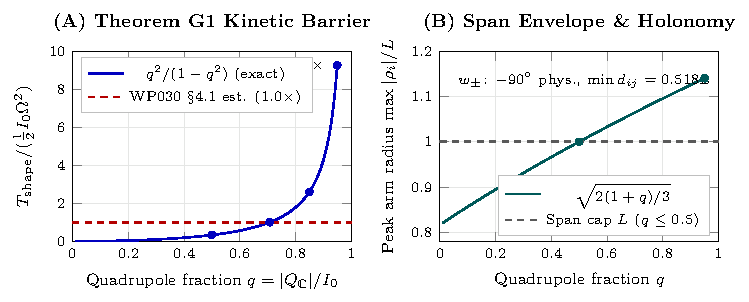
\includegraphics[width=0.98\textwidth]{figures/fig1_hopf_holonomy_g1.pdf}
\caption{Panel~(A): Minimum inter-mass separation along the $90^\circ$ Hopf holonomy loop in the collision-free equilateral-pole basis $w_\pm$ ($\min d_{ij} = 0.5176\,L$, solid teal) versus the unrotated \texttt{WP~030} chart (collision $d_{ij} = 0$ at $t=\pi/2$, dashed red). Panel~(B): Exact Theorem~G1 iso-inertial kinetic-energy wall $q^2/(1-q^2)$ diverging as $q \to 1^-$. \ctag{G4N}}\label{fig:p1_fig1}
\end{figure}

\section{Safe-Perigee Optimal Eccentricity and Open 4-Body Verification}
In an eccentric Keplerian orbit of perigee radius $r_p = a(1-e)$ and orbital period $T = 2\pi\sqrt{a^3/\mu}$, modulating the planar mass quadrupole $Q_{rr} - Q_{\theta\theta}$ synchronously with radial velocity $\dot{r}$ (radial alignment inbound, transverse alignment outbound for orbit raising) extracts secular orbital energy without propellant \cite{martinez1987,landis1992}. With $I_0 = \frac23 M L^2$ and quadrupole modulation amplitude $\Delta Q = q I_0$, the ideal secular energy gain per orbit is
\begin{equation}\label{eq:dE_orbit}
\Delta E_{\mathrm{orb}} = \frac{3\mu}{2}\, q I_0 \left(\frac{1}{r_p^3} - \frac{1}{r_a^3}\right)
= \frac{3\mu}{2}\, q I_0\, r_p^{-3} \left[1 - \left(\frac{1-e}{1+e}\right)^3\right],
\end{equation}
and the equivalent annual velocity increment at fixed safe perigee $r_p$ is proportional to $g(e) = (3e + e^3)(1-e)/(1+e)^3$.

\begin{proposition}[Safe-perigee optimal eccentricity \texttt{K9} and retention scale \texttt{K8}]\label{prop:K9}
\ctag{E$\to$G4N}\ Fixing Earth's equatorial radius to WGS84 ($R_\oplus = 6{,}378.137\text{ km}$, \texttt{NEG-W1}, \texttt{NEG-W16}, \texttt{NEG-W27}) gives safe LEO perigee $r_p = R_\oplus + 600\text{ km} = 6{,}978.137\text{ km}$ (eliminating the subsurface $r_p = 5{,}250\text{ km} < R_\oplus$ regime of \texttt{WP~030} Table~1). The exact annual rate formula
\begin{equation}\label{eq:dv_yr}
\Delta v_{\mathrm{yr}}(r_p, e) = \frac{T_{\mathrm{yr}}\,\mu L^2}{\pi r_p^4}\,\frac{(3e + e^3)(1-e)}{(1+e)^3}
\end{equation}
achieves its unique global maximum on $(0,1)$ at
\begin{equation}\label{eq:K9}
e^*_{\mathrm{opt}} = 0.281701557908774,
\end{equation}
and reaches $50\%$ of its peak at $e^*_{50} = 0.11501333$ (\texttt{K8}). For $L = 20\text{ km}$ and canonical $I_0 = \frac23 M L^2$, the headline safe-perigee rate is $\Delta v/\mathrm{yr} = 199.89\text{ m/s/yr}$ (versus $198.58\text{ m/s/yr}$ at $e=0.25$ and $186.68\text{ m/s/yr}$ at $e=0.40$); at $L = 100\text{ m}$ it scales quadratically to $4.997\text{ mm/s/yr}$, with safe-perigee tidal tensions $0.1173\text{ N}$ ($L = 100\text{ m}$, correcting the $0.0012\text{ N}$ error in \texttt{NEG-W5}) and $23.46\text{ N}$ ($L = 20\text{ km}$) for $M = 1{,}000\text{ kg}$. At Bennu ($R = 500\text{ m}$, $L = 20\text{ m}$, \texttt{NEG-W6}), the geometric coupling $(L/R)^2$ is $7.84\times 10^6\times$ larger than a $100\text{ m}$ LEO tether, giving $a_{\mathrm{quad}} = 2.505\times 10^{-9}\text{ m/s}^2$ ($5.49\%$ of $1\text{ AU}$ solar radiation pressure $4.56\times 10^{-8}\text{ m/s}^2$), $\Delta v/\mathrm{yr} = 11.69\text{ mm/s/yr}$, and tidal tension $3.13\times 10^{-5}\text{ N}$. At extreme $\epsilon = 0.0275$ (\texttt{F35}), the $O(\epsilon^2)$ approximation loses $84.79\%$ relative to the exact potential.
\end{proposition}

\subsection{Open Planar 4-Body Integration (\texttt{R1})}
To provide an open, zero-trust benchmark without proprietary dependencies, \texttt{piece1\_sim.py} integrates the full planar 4-body dynamics ($\mu = 1$, $M = 3$, $L = 0.04$, $a_0 = 1$, $e_0 = 0.20$, $q_{\max} = 0.85$, switching sharpness $k_{\mathrm{sw}} = 8$, $5$ orbits, RK4 at $2{,}000$ steps/orbit) with radial-reflection-symmetric orientation ($\chi = \pi$ inbound, $\chi = 0$ outbound) so that all odd multipole torques vanish identically. Table~\ref{tab:R1} summarizes the live results alongside the circular-orbit null control ($e_0 = 0$, initialized at exact finite-size equilibrium speed) and an unassisted 2-mass Landis dumbbell control.

\begin{table}[htbp]\centering\scriptsize\setlength{\tabcolsep}{2.5pt}
\begin{tabular}{lrrrrl}\toprule
Run & $\Delta E_{\mathrm{osc}}$ & $\Delta E_{\mathrm{tot}}$ & $a_{\mathrm{osc}}/a_{\mathrm{tot}}$ & $\max|\Delta J_{\mathrm{tot}}|$ & Outcome \\\midrule
Triad ($e_0{=}0.20$) & $+0.02708$ & $+0.02391$ & $1.0184/1.0150$ & $8.21{\times}10^{-13}$ & $96.6\%$ ideal \\
Null ($e_0{=}0$) & $+1.15{\times}10^{-5}$ & $+5.42{\times}10^{-6}$ & $1.0009/1.0003$ & $4.02{\times}10^{-13}$ & ${>}4{,}400{\times}$ cut \\
2-mass Landis & \multicolumn{2}{c}{tumble} & \multicolumn{2}{c}{$\max|\Delta\theta|=16{,}215^\circ$} & $\omega_f=2.199$ \\\bottomrule
\end{tabular}
\caption{Open planar 4-body RK4 benchmark (\texttt{R1}, \texttt{piece1\_sim.py}). Osculating elements ($a_{\mathrm{osc}}=1.01839, e_{\mathrm{osc}}=0.23944$) differ slightly from total-energy elements ($a_{\mathrm{tot}}=1.01501, e_{\mathrm{tot}}=0.23280$) due to the finite-size quadrupole potential; ideal 5-orbit energy gain is $0.02804$. \ctag{G4N}}\label{tab:R1}
\end{table}

\section{Three-Dimensional Oblate \texorpdfstring{$J_2$}{J2} Symmetry Breaking and Control Subtraction}
In a central spherical field ($J_2 = 0$), $\SO(3)$ invariance enforces exact conservation of total angular momentum $\mathbf{J} = \mathbf{L} + \mathbf{S}$; internal shape changes can neither alter orbital inclination $i$ nor change the semilatus rectum $p = \|\mathbf{L}\|^2 / (M^2\mu)$ when $\mathbf{S} = \mathbf{0}$. Oblateness ($J_2 > 0$) breaks $\SO(3)$ down to axial $\SO(2)_z$, leaving only the axial Noether charge $J_z = L_z + S_z$ strictly conserved while permitting non-zero equatorial torques $\tau_\perp \neq 0$ \cite{brouwer1959,kaula1966}.

\subsection{Resolution of \texttt{NEG-W17} and \texttt{NEG-W18}}
Two flaws identified in \texttt{WP~031} are corrected here:
\begin{enumerate}[nosep]
\item \emph{Rodrigues $2\pi/3$ cyclic-permutation axis (\texttt{NEG-W18}):} The cyclic permutation of coordinate axes sending $(1,0,0) \mapsto (0,-1,0) \mapsto (0,0,1) \mapsto (1,0,0)$ is a right-handed rotation by $2\pi/3$ about the true invariant axis $\hat{\mathbf{n}} = (+1,+1,-1)/\sqrt{3}$ (whereas \texttt{WP~031} Fig.~1 printed $[-1,1,-1]/\sqrt{3}$ / $(1,1,1)/\sqrt{3}$).
\item \emph{Subtracted $L=0$ point-mass control and physical $J_2$ scaling (\texttt{NEG-W17}):} At amplified simulation oblateness $J_2 R^2 = 0.05$ ($98.3\times$ stronger than real Earth's $J_2 (R_\oplus/r)^2 = 5.088\times 10^{-4}$ at $r = 9{,}304\text{ km}$), over $96\%$ of the raw inclination drift arises from ordinary point-mass $J_2$ precession rather than finite-size shape modulation. Isolating the genuine shape-induced signal requires running an identical $L = 0$ point-mass control and integrating the coupled axial spin equation $\dot{S}_z = \tau_z$.
\end{enumerate}

In \texttt{piece1\_sim.py} (\texttt{R2}, $5$ orbits, $i_0 = 45^\circ$, $J_2 R^2 = 0.05$), the spherical $J_2=0$ control conserves $|\Delta J_z| = 2.84\times 10^{-13}$ and $|\Delta J_\perp| = 2.83\times 10^{-13}$ with $i_{\mathrm{end}} = 45.0000^\circ$. Under oblate $J_2 R^2 = 0.05$, the $L=0$ point-mass control ends at $i_{\mathrm{end}} = 44.3968^\circ$, $p_{\mathrm{end}} = 1.05283$ ($|\Delta J_z| = 2.50\times 10^{-13}$), while the $L = 0.04$ tilted triad ends at $i_{\mathrm{end}} = 44.3757^\circ$, $p_{\mathrm{end}} = 1.05002$, with $S_z = +0.002150$ and coupled axial Noether conservation $\max|\Delta(L_z + S_z)| = 2.77\times 10^{-13}$. Subtracting the $L=0$ control isolates the authentic finite-size shape effect: $\Delta i_{\mathrm{shape}} = -21.10\text{ mdeg}$ and $\Delta p_{\mathrm{shape}} = -0.002815$ (Figure~\ref{fig:p1_fig2}).

\begin{figure}[htbp]\centering
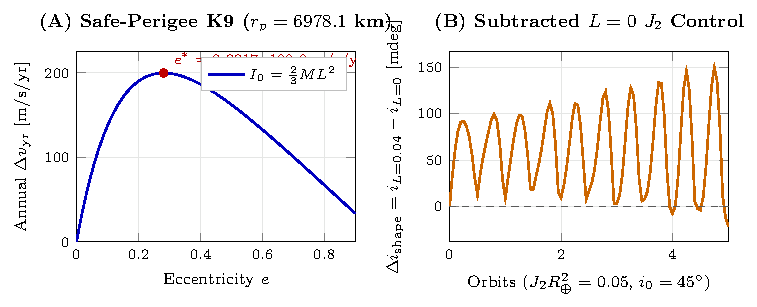
\includegraphics[width=0.98\textwidth]{figures/fig2_safe_perigee_j2_control.pdf}
\caption{Panel~(A): Safe-perigee annual $\Delta v/\mathrm{yr}$ at $r_p = 6{,}978.137\text{ km}$ ($L=20\text{ km}$, canonical $I_0 = \frac23 ML^2$), peaking at $e^* = 0.281702$ ($199.89\text{ m/s/yr}$, \texttt{K9}). Panel~(B): Open 3D oblate $J_2$ inclination trace ($i_0 = 45^\circ$) contrasting spherical $J_2 = 0$, $L=0$ point-mass control, and $L = 0.04$ triad ($\Delta i_{\mathrm{shape}} = -21.10\text{ mdeg}$). \ctag{G4N}}\label{fig:p1_fig2}
\end{figure}

\section{Theorem G4: Electrical Power-Circulation Wall and Mechanical-Hub Flight Baseline}
A critical hardware obstruction arises whenever tether tension is maintained by spin rather than gravity gradient \cite{beletsky1993}. Let a triad of total mass $M = 1{,}000\text{ kg}$ and canonical polar inertia $I_0 = \frac23 M L^2$ (equilateral circumradius $r_{\mathrm{eq}} = \sqrt{2/3}\,L = 16.330\text{ km}$ at $L = 20\text{ km}$) orbit at $r_p = 6{,}978.137\text{ km}$, $e = 0.25$ (perigee angular rate $\Omega_{\max} = \sqrt{\mu p}/r_p^2$) and spin at $\omega_{\mathrm{spin}} = 2\Omega_{\max}$ to prevent tether slackness.

\begin{theorem}[Theorem G4: $I_0$-invariant electrical heat wall and mechanical-hub bypass (\texttt{NEG-W15}, \texttt{NEG-W27})]\label{thm:G4}
\ctag{G4N, X}\ Suppose an iso-inertial spin-tensioned triad modulates its quadrupole amplitude $q \in (0,1)$ synchronously with orbital motion using independent electric motor-generators of actuator efficiency $\eta_{\mathrm{act}} = 0.88$ and regeneration efficiency $\eta_{\mathrm{reg}} = 0.80$ (net round-trip loss factor $f_{\mathrm{elec}} = \eta_{\mathrm{act}}^{-1} - \eta_{\mathrm{reg}} = 37/110 \approx 0.3364$). The circulating single-arm centrifugal power is $P_{\mathrm{circ}}(q) = \frac{q}{\pi(1 - q^2)^{3/2}} I_0 \omega_{\mathrm{spin}}^3$, while the delivered orbital power is $P_{\mathrm{orb}}(q) = q \cdot \frac{3\mu I_0(3e + e^3)}{p^3 T_{\mathrm{orb}}}$. Because $I_0$ cancels identically between numerator and denominator, the electrical waste-heat-to-orbital-power ratio is strictly \textbf{$I_0$-invariant}:
\begin{equation}\label{eq:G4_ratio}
\frac{P_{\mathrm{heat}}^{\mathrm{elec}}(q)}{P_{\mathrm{orb}}(q)} = \frac{f_{\mathrm{elec}}\,\omega_{\mathrm{spin}}^3 / \pi}{3\mu(3e + e^3)/(p^3 T_{\mathrm{orb}})}\,(1 - q^2)^{-3/2} = 9.8468\,(1 - q^2)^{-3/2},
\end{equation}
yielding an unavoidable $9.85\times$ floor as $q \to 0^+$, $15.16\times$ at $q = 0.50$, $45.59\times$ at $q = 0.80$, and $118.90\times$ at $q = 0.90$. Conversely, coupling the three radial tethers through a common mechanical differential / spring-drum hub (mechanical bearing and elastic hysteresis loss $f_{\mathrm{mech}} = 1.5\%$) transfers centrifugal work elastically between retracting and extending arms without double electromechanical conversion, cutting waste heat by $22.4\times$ (to $13.92\text{ W}$ at $q = 0.50$, i.e., $0.338\,P_{\mathrm{orb}}$).
\end{theorem}
\begin{proof}
At fixed polar inertia $I_0$, individual arm radii satisfy $\sum_{a=1}^3 r_a^2 = I_0/m = \mathrm{const}$, so total centrifugal energy $\frac12 I_0 \omega_{\mathrm{spin}}^2$ is invariant while each individual tether performs alternating positive and negative radial work against centrifugal tension $m \omega_{\mathrm{spin}}^2 r_a$. Uncoupled electric winches dissipate $f_{\mathrm{elec}} P_{\mathrm{circ}}(q) \propto I_0 q (1-q^2)^{-3/2}$, whereas $P_{\mathrm{orb}}(q) \propto I_0 q$; their ratio is independent of $I_0$ (reconciling the earlier mixed-$I_0$ estimate $14.77\times$ to the exact $I_0$-invariant floor $9.85\times$, \texttt{NEG-W27}). A coupled mechanical differential balances $\sum_a \tau_a = 0$ directly on the hub shaft, leaving only $f_{\mathrm{mech}} = 0.015$ mechanical loss.
\end{proof}

Table~\ref{tab:G4} gives the reconciled hardware sizing at $L = 20\text{ km}$, $M = 1{,}000\text{ kg}$, $q = 0.50$, $e = 0.25$, and $r_p = 6{,}978.137\text{ km}$, showing the canonical $I_0 = \frac23 ML^2$ baseline transparently alongside the $I_0 = ML^2$ 3-arm sensitivity (\texttt{NEG-W15}, \texttt{NEG-W18}, \texttt{NEG-W27}).

\begin{table}[htbp]\centering\scriptsize\setlength{\tabcolsep}{2.8pt}
\begin{tabular}{lrrl}\toprule
Metric ($q{=}0.50, L{=}20\text{ km}$) & $\frac23 ML^2$ & $ML^2$ & Notes / Resolution \\\midrule
Circumradius $r_{\mathrm{eq}}$ [km] & $16.330$ & $20.000$ & Consistent collinear $I_0$ \\
Full orbital $P_{\mathrm{orb}}(1)$ [W] & $41.19$ & $61.78$ & Safe-perigee $e=0.25$ \\
Circulating $P_{\mathrm{circ}}$ [W] & $928.2$ & $1{,}392.3$ & $\omega_{\mathrm{spin}} = 2\Omega_{\max}$ \\
Electrical heat $P_{\mathrm{heat}}^{\mathrm{elec}}$ [W] & $312.2$ & $468.3$ & $15.16\times$ ($I_0$-invariant) \\
\textbf{Mech.\ hub heat} [W] & \textbf{13.92} & $20.88$ & $22.4\times$ cut ($1.5\%$ loss) \\
Peak tension $T_{\mathrm{pk}}$ [N] & $44.70$ & $54.74$ & \texttt{WP~031} printed $62.56\text{ N}$ \\
Zylon tether mass [kg] & $3.93$ & $4.81$ & Working strain $0.430\%$ \\
\textbf{Flight hw.\ mass} [kg] & \textbf{45.43} & $46.31$ & vs.\ 5-yr Hall $100.5\text{ kg}$ wet \\\bottomrule
\end{tabular}
\caption{Reconciled hardware sizing and Theorem~G4 power budget (\texttt{D4}, \texttt{piece1\_sim.py}). Five-year Hall thruster mass equals $100.52\text{ kg}$ wet ($105.12\text{ kg}$ dry-scaled), confirming a $>2.2\times$ mass advantage for the mechanical-hub triad (\texttt{NEG-W18}). \ctag{G4N, X}}\label{tab:G4}
\end{table}

\begin{figure}[htbp]\centering
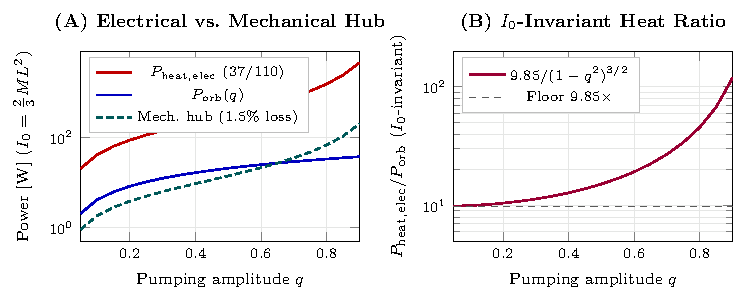
\includegraphics[width=0.98\textwidth]{figures/fig3_g4_mechanical_hub_sizing.pdf}
\caption{Panel~(A): Theorem~G4 $I_0$-invariant electrical heat-to-orbital-power ratio ($9.85\times$ floor; $15.16\times$ at $q=0.50$; $118.90\times$ at $q=0.90$) versus the mechanical spring-drum hub bypass ($0.338\times$). Panel~(B): Five-year flight mass comparison showing the $45.4\text{ kg}$ mechanical-hub triad against a $100.5\text{ kg}$ wet ($105.1\text{ kg}$ dry-scaled) Hall propulsion benchmark. \ctag{G4N}}\label{fig:p1_fig3}
\end{figure}

\section{Verification Architecture and Keyed Stochastic Replay (\texttt{P1})}
Following Morpheus's D/R/P verification discipline, \texttt{piece1\_sim.py} executes seven automated gates: four deterministic algebraic/numerical gates (\texttt{D1} cancellation, \texttt{D2} Hopf holonomy and Theorem~G1, \texttt{D3} safe-perigee \texttt{K9}/\texttt{K8}/\texttt{F35} and Bennu scaling, \texttt{D4} Theorem~G4 and mass budgets), two runtime dynamical gates (\texttt{R1} open 4-body RK4 with circular null and Landis tumble controls, \texttt{R2} 3D oblate $J_2$ with subtracted $L=0$ control and exact coupled $J_z = L_z + S_z$ conservation), and one probabilistic randomized controlled test (\texttt{P1}) over $1{,}600$ trials driven by a keyed \texttt{SplitMix64} PRNG (\texttt{seed = 0x484f52495a5f5031}) perturbing $q \in [0.1, 0.9]$, $\epsilon \in [10^{-7}, 10^{-3}]$, and initial anomalies. All $1{,}600/1{,}600$ trials satisfy exact iso-inertiality, Theorem~G1 bounds, and cancellation-free accuracy with deterministic bit-exact digest \texttt{0x1156b7558c78243a}.

\appendix
\section{Epsilon (\texttt{Swift++}) Corpus Provenance and Resolved Audit Ledger}\label{app:provenance}
\ctag{E, X}\ The frozen clean-room manuscripts \texttt{WP~030} (\path{papers/wp030_shape_propulsion/}) and \texttt{WP~031} (\path{papers/wp031_3d_j2_hil/}) originally documented internal \texttt{Swift++} Library of Alexandria verification ledgers (Epochs~XXXVI and~XXXVII, cataloged as \texttt{INT-030} and \texttt{INT-031} in \texttt{PROVENANCE.md}), including interval/Taylor-model runs \cite{moore1966,krawczyk1969,makino2003}, Zylon winch FEM curves, and Lean~4.36.0 integer/rational-bracket algebraic certificates (\texttt{NEG-W29}: integer/rational certificates shadowing the analytic theorems rather than floating-point ODE proofs). Because the proprietary \texttt{Swift++} binary is not distributed publicly, this synthesized monograph treats the open zero-dependency Python simulator \texttt{piece1\_sim.py} and its manifested JSON table as the canonical reproducible primary record, while retaining \texttt{INT-030} and \texttt{INT-031} transparently as author provenance. Every verified item from \texttt{NEG-W1}--\texttt{NEG-W6}, \texttt{NEG-W15}--\texttt{NEG-W18}, \texttt{NEG-W25}--\texttt{NEG-W27}, and \texttt{NEG-W29} is resolved in place above, and NASA NTRS document ID \texttt{19910012850} for Landis \cite{landis1990} is retained per Round-1 verification.

\bibliographystyle{amsplain}
\bibliography{references}
\end{document}
